\chapter{Results}
\label{cap:Results}
The evaluation of the piano recordings yielded promising results, offering valuable insights into the reliability and consistency of the rater system. The slopes and intercepts of the piano progress varied strongly among the participants, which is expected given their diverse individual backgrounds. The results are categorized into four main areas of evaluation: the rater system, the progress of piano playing, the progress in other musical abilities, and the exploration of a potential general \textit{musicality} factor.


\section{Rater System}

With the double rated evaluations the Intraclass Correlation Coefficient (ICC) values were computed to determine the level of agreement and consistency among the raters' evaluations. Table \ref{fig:icc} presents the ICC values for each rater across the six variables.

\begin{figure}[h]
	\centering
	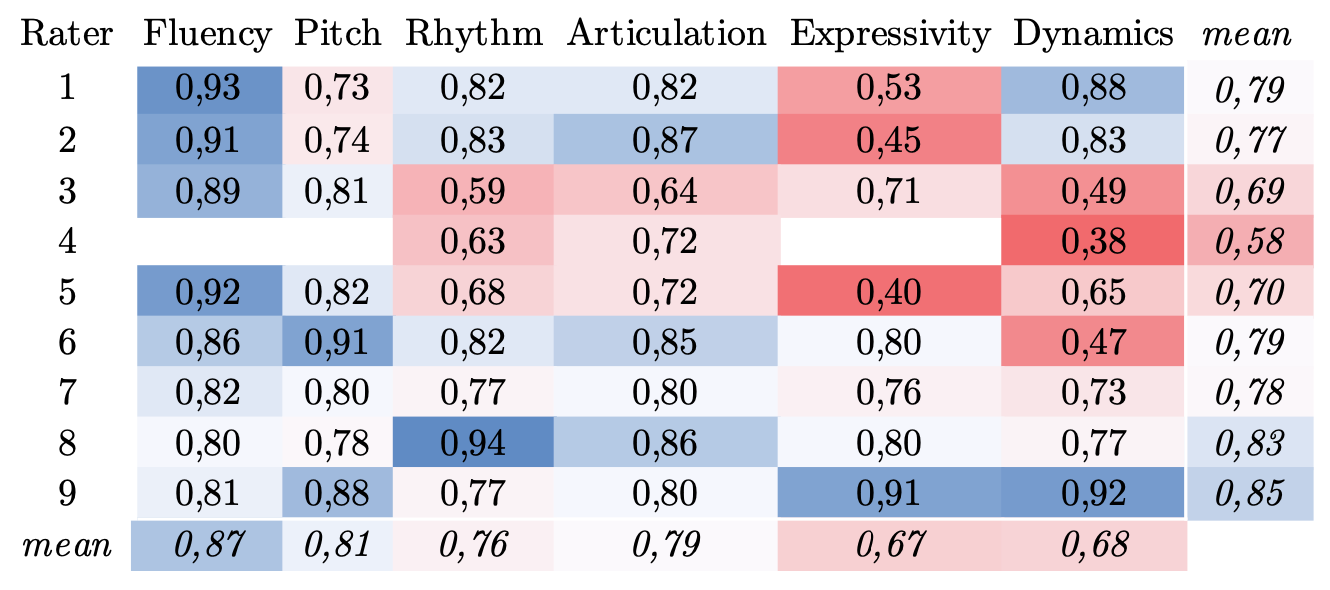
\includegraphics[width=12cm,height=10cm,keepaspectratio]{ICC}
	\caption{ICC Values of Each Rater for Each Variable}
	\label{fig:icc}
	\textcolor{blue}{> .9; excellent}, \textcolor{lightblue}{.75 - .9; good }, \textcolor{red}{.5 - .75; moderate }, \textcolor{purple}{> .5; poor reliability} \cite{Koo2016}.
\end{figure}

The ICC values indicated varying degrees of agreement among the raters for each variable. For fluency, the ICC values ranged from 0.803 to 0.931, indicating a high level of consistency among the raters' assessments. Similarly, pitch exhibited strong agreement among the raters, with ICC values ranging from 0.733 to 0.91. Rhythm evaluations also demonstrated a high level of agreement, with ICC values ranging from 0.586 to 0.943. Articulation was assessed with moderate to high reliability, as indicated by ICC values ranging from 0.64 to 0.858. Expressivity showed moderate agreement among the raters, with ICC values ranging from 0.404 to 0.907. The evaluations of dynamics exhibited the greatest variability among the raters, with ICC values ranging from 0.378 to 0.915. Overall, the results suggest that the raters demonstrated good to strong consistency in evaluating fluency, pitch, rhythm, and articulation. However, there was more variability in the assessments of expressivity and dynamics.

The ICC values reveal considerable variability in consistency among the raters. For instance, Rater 8 and Rater 9 demonstrate higher reliability compared to Rater 3 and Rater 4. Despite analyzing factors such as age, years of piano practice or teaching, no clear explanations for these differences were found, likely due to the small group size and alignment of raters in these factors. Furthermore, no differences were observed between different university degrees, such as music educators and musicians, in terms of rating.
In the subsequent analysis, the ratings were weighted based on the ICC values per rater and variable. This approach ensured that raters with higher consistency had a greater impact on the analysis of musical performance compared to raters with lower ICC values.

The Interrater correlation also showed moderate to high reliability among all raters (see figure \ref{fig:heat}). Among the raters no outlier could be found. As shown in table \ref{tab:interrater} the correlation coefficients are between 0.78 and 0.93. Expressivity shows the lowest reliability of 0.78, still being in a good range. The raters agreed most on fluency as shown by the correlation score of 0.93. Articulation and Pitch follows directly. 
\begin{table}[h]
	\centering
	\caption{Interrater Coefficients for Each Variable }
	\label{tab:interrater}
	\renewcommand{\arraystretch}{1.2}
	\vspace{\medskipamount}
	\begin{tabular}{l|cccccc}
		&    Articulation	& Dynamics & Rhythm & Fluency & Pitch & Expressivity     \\
		\hline
		Interrater Coefficient       &  0.92 & 0.87 & 0.87 & 0.90 & 0.93 & 0.78\\
	\end{tabular}\par
	\vspace{\medskipamount}
\end{table}

\section{Piano Progress}
\label{cap:PianoProgress}

neues, richtiges bild!

\begin{figure}[h]
	\centering
	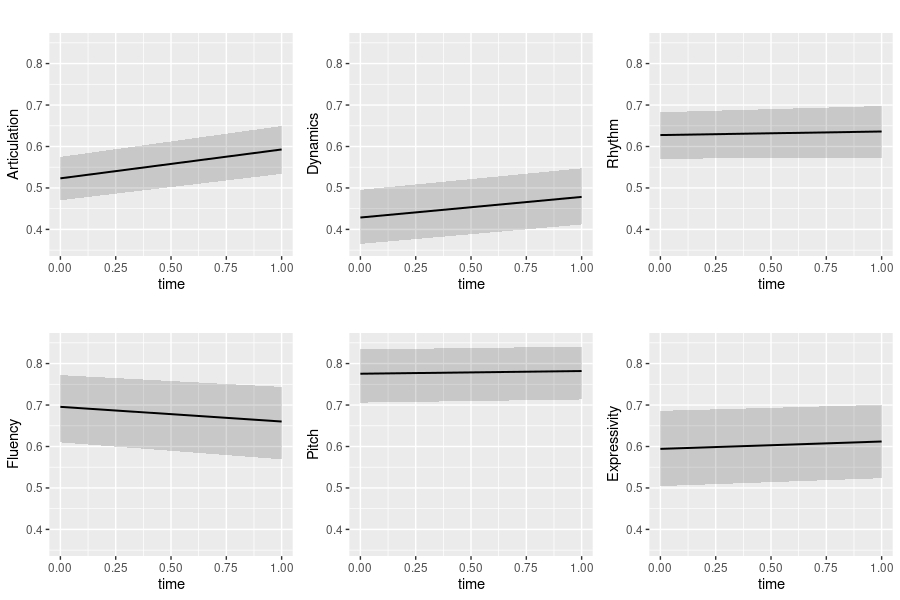
\includegraphics[width=15cm,height=10cm,keepaspectratio]{pred_vals}
	\caption{Predicted Values over time}
	\label{fig:PredVals}
\end{figure}

The models convergered with a Rhat-value of 1.0, indicating a satisfactory convergence of the Markov Chain Monte Carlo algorithm used for estimation. The analysis of piano playing progress across the six variables articulation, dynamics, rhythm, fluency, pitch, and expressivity, revealed generally strong variations in slopes and intercepts. Examining the changes in these variables over time, various patterns emerged (see Figure \ref{fig:PredVals}). Notably, while articulation showed the strongest improvement, the score for fluency decreased. Below, a detailed analysis of each variable is presented. 

\minisec{Articulation}
 The intercept for articulation is 0.52 (95\% CI [0.47, 0.59]), indicating a moderate level of articulation proficiency at the beginning. Over time, there was a clear positive time effect (0.43, [0.18, 0.68]), suggesting that participants' articulation skills improved during the intervention. On average, the subjects displayed a 10,6\% improvement in articulation as a result of the intervention, starting from 49.6\% improving to 60.2\%.
Although the effect values for demographic factors are relatively small, trends can be observed in relation to articulation scores. Participants with higher income (0.23, [0.02, 0.43]) displayed higher articulation scores initially. Similarly, participants with higher cognitive reserve (0.10, [-0.11, 0.30]), higher educatioin (0.15, [-0.05, 0.35]) and higher CogTel scores (0.13, [-0.07, 0.33]) exhibited higher articulation scores initially. Although the 95\% CI of cognitive reserve, education and CogTel include zero, the variables have a 82\%, 93\% and 90\% probability of positively affecting musical performance. The goldMSI categories showed no effect on participants' initial articulation performance. 
To understand if the effect of demographic factors on articulation changed over time, we examined the interaction between each demographic factor and time. Participants who spent more time on their homework were 93\% more likely to show improvement over time (0.18, [-0.06, 0.41]). It is 97\% likely that younger participants also improved more (-0.20, [-0.41, 0.01]).
Participants with self-reported lower levels of musical engagement improved more in articulation scores during the intervention (-0.29, [-0.51, -0.08]). The effect of emotions towards music and singing abilites on articulation over time was also clearly negative (-0.23, [-0.44, -0.02]; -0.28, [-0.45, -0.05]). Perceptual abilities (-0.1, [-0.31, 0.11]) and musical training (-0.12, [-0.33, 0.10]) had a negative effect on articulation during the intervention, both being 85\% likely to be negative. Participants with lower scores in these areas showed more increases in articulation compared to those with higher scores. General sophistication had a negative effect on articulation over time (-0.19, [-0.34, -0.05]). Participants with higher levels of general sophistication displayed a decrease in articulation scores during the intervention.
After twelve months of intervention, participants with higher CogTel (0.15, [-0.03, 0.39]) and higher income (0.21, [-0.03, 0.45])  were 90\% and  96\% likely to have higher articulation scores on the more difficult version of "Ode to Joy". Additionally, homework was 95\% likely to have a positive impact (0.21, [-0.04, 0.47]).

\minisec{Dynamics}
The intercept for piano performance in terms of dynamic quality is 0.44 ([0.38, 0.52]), indicating a relatively low baseline performance. However, the time effect of 0.38 ([0.08, 0.67]) suggests a positive development over time, indicating that participants showed improvement in dynamics during the intervention. On average, the participants' dynamic skill improved by 8.9\% over the course of the intervention, from  39.6\% to 48.5\%. 
Initially, education had an impact on the dynamic scores. Participants with higher education scored generally better in the easy version of "Ode to Joy" in the first measurement (0.19 [0.00, 0.38]). In addition, participants from Geneva were likely to have better dynamic quality (0.13, [-0.07, 0.32]), with a 90\% probability of the effect values being positive. Participants who self-reported having a high score regarding their emotions towards music scored clearly better than the others (0.24, [0.04, 0.42]).
Over time, the younger participants were 95\% likely to improved more (-0.22, [-0.47, 0.04]). Participants with more cognitive reserve seemed to show greater improvements (0.17, [-0.09, 0.43]), but the effect was not very credible (91\% of all effect values are positive). Again, participants with less musical emotion improved more (-0.37, [-0.61, -0.13]). A negative trend (95\% of effect values were negative) was observed regarding participants with low musical engagement, as they showed more improvement than others. 
In the more difficult version of "Ode to Joy", participants with higher cognitive reserve scores performed better (0.28, [0.06, 0.50]). Furthermore, female participants were 90\% and participants with higher CogTel scores 93\% likely to reach higher dynamic skills. 

\minisec{Rhythm}
The intercept for rhythmic skills is 0.63 [0.52, 0.70], indicating a moderate baseline performance compared to other variables. Rhythmic skills did not change over time (-0.01, [-0.16, 0.28]).
Regarding demographic factors, the analysis revealed that men exhibited higher rhythmic skills at the beginning (0.25,  [0.01, 0.49]). Additionally, participants with higher income (0.19, [-0.02, 0.39]), higher CogTel scores (0.20, [-0.01, 0.40]), less age (-0.16, [-0.35, 0.05]), and higher musical engagement (0.12, [-0.08, 0.31]) were most likely to show higher rhythmic scores. Cognitive reserve also had a positive effect on rhythmic skills (0.38, [0.14, 0.61]).
Over time, lower educated participants were 90\% sure to improve more (-0.13,[-0.32, 0.07]). Participants with lower income (-0.15, [-0.36, 0.05]) and lower CogTel scores (-0.15, [-0.35, 0.05]) were 93\% likely to improve more. Emotions towards music were 90\% likely to have a negative effect (-0.13, [-0.33, 0.07]), suggesting an increase in rhythmic skills over time for participants with less emotions. 
At difficulty level 1, participants with higher cognitive reserve were associated with better rhythmic scores (0.20, [-0.01, 0.42]), as well as higher perceptual abilities (0.22, [0.02, 0.43]), and general sophistication (0.17, [-0.05, 0.38]).

\minisec{Fluency}
The intercept for fluency is 0.71 [0.62, 0.78], indicating a relatively high baseline performance. However, there is a  likely negative time effect of -0.09 [-0.32, 0.14], suggesting a negative trend over 2.4\% in fluency over the intervention period.
Regarding demographic factors, being male had a positive effect (0.25, [0.01, 0.49]). Participants from Hanover also had higher fluency scores (-0.18, [-0.43, 0.07]), with a 92\% probability of being real. Higher cognitive reserve had a strong positive effect on fluency (0.38, [0.14, 0.61]), and no effect was observed for goldMSI categories.
While musical training had a possible but small positive effect on fluency over time (0.13, [-0.07, 0.33]), emotions had a possible but negative effect on fluency over time (-0.18, [-0.38, 0.02]), being 90\% and 96\% likely to be positive or negative, respectivly.
At difficulty level 1, being male had a 92\% likely positive effect on fluency (0.14, [-0.15, 0.45]). Participants with higher cognitive reserve were rated to play more fluent (0.32, [0.01, 0.62]) and again participants from Hanover scored higher (0.12, [-0.08, 0.33]), with the effect being 92\% likely to be positive. Higher perceptual abilities (0.28, [-0.01, 0.57]) and higher general musical sophistication (0.20, [-0.10, 0.51]) showed postive effects being 97\% and 91\% likely on fluency. 


\minisec{Pitch}
The analysis of pitch data revealed a high baseline performance, with an intercept of 0.78 [0.71, 0.84]. Participants demonstrated a high starting level of pitch accuracy. Over the intervention period, there was no a trend of positive improvement in pitch (0.16, [-0.14, 0.46]).
At baseline, CogTel and cognitive reserve had positive effects on pitch, with coefficients of 0.23 [0.00, 0.47] and 0.27 [0.05, 0.50], respectively.
Participants with lower CogTel scores 90\% likely improved more (-0.13, [-0.33, 0.08]). Cognitive reserve showed a negative effect, indicating that participants with higher cognitive reserve demonstrated less improvement in pitch accuracy (-0.28, [-0.56, -0.00]). Similarly, musical engagement was associated with reduced pitch improvement (-0.26, [-0.54, -0.03]). Singing abilities (-0.21, [-0.50, 0.08]) also had a 92\% likely negative effect on pitch improvement. Moreover, emotions towards music showed a strong negative effect on pitch improvement (-0.37, [-0.65, -0.10]). 
At difficulty level 1, age showed a 95\% likely negative effect (-0.21, [-0.45, 0.03]), indicating that younger participants achieved higher pitch scores. Cognitive reserve had a positive effect, with an effect size of 0.26 [0.02, 0.51], indicating that participants with higher cognitive reserve scores performed better on pitch evaluation. Also participants from Hanover were 94\% to score higher pitch scores (-0.19, [-0.43, 0.05]).

\minisec{Expressivity}
The analysis of expressivity data revealed a moderate baseline performance, with an intercept of 0.61 [0.52, 0.71]. Over the intervention period, there was a small likely improvement in expressivity, as evidenced by a time effect of 0.15 [-0.05, 0.34].
Higher education and higher CogTel scores had a small positive with a probability of 91\% influence on expressivity skills after three months (both 0.12, [-0.06, 0.3]). Cognitive reserve was 97\% likely to have a positive impact (0.16, [-0.01, 0.33]).
The time spent on homework had a clear positive effect on the development of expressivity performance (0.21, [0.04, 0.39]).
Participants with lower emotion towards music demonstrated 94\% likely better expressiveness (-0.13, [-0.30, 0.03]).
Additionally, higher cognitive reserve showed a strong positive effect on expressivity at the more challenging version of "Ode to Joy" (0.25, [0.05, 0.45]), indicating that participants with more cogntive reserve sophistication performed better in expressivity. Also men were 91\% likely to score higher on expressivity (0.14, [-0.07, 0.34]). Partcipants with higher perceptual abilities reached higher expressivity scores in the more challenging version after 12 months (0.24, [0.05, 0.44]). Similarly, participants with higher general sophistication were 94\% likely to score higher (0.17, [-0.04, 0.38]).


%in discussion?
Conclusively, the participants made clear improvements in articulation and very likely improvements in dynamics, whereas pitch, expressivity, and rhythm did not change over time. Moreover, fluency likely decreased over time. For and overview of the coefficents of all predictors impacting piano performance at different levels of difficulty, see Table \ref{tab:preds}. Only a few demographics could be confirmed to potentially predict the performance in various piano-related skills. Overall, it could be suggested that younger people with more cogntive reserve and a higher CogTel achieve higher scores in different aspects of piano performance. While people who describe themselves to have more emotions toward music, more singing and perceptual abilities, and a higher general musical sophistication reach higher scores when performance is tested, those who have less of all improve better over time. To generalize these observations the analysis is repeated on a potential \textit{musicality} factor which could be extracted through factor analysis. 

\section{One General \textit{Musicality} Factor}

faktorenanalyse mit sem path and predictors?


Three separate factor analyses were conducted revealing patterns of shared variance that contribute to participants' overall musical performance: one at the baseline with the easy version of "Ode to Joy" ($FA_{0,0}$), another after 12 months of intervention with the easy version ($FA_{1,0}$), and the third after the intervention with the more challenging version of "Ode to Joy" ($FA_{1,1}$).
\begin{figure}[h]
	\centering
	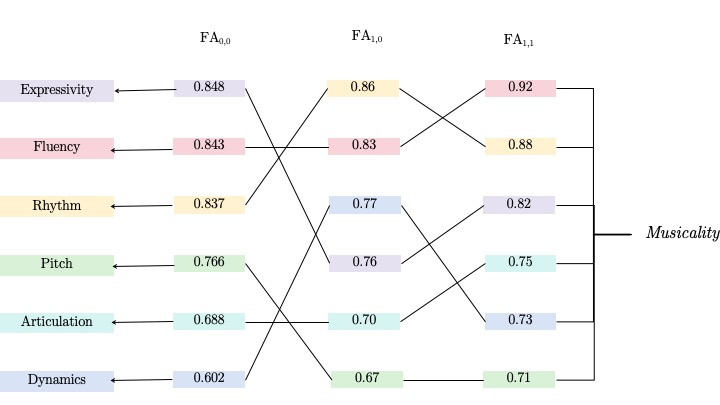
\includegraphics[width=15cm,height=10cm,keepaspectratio]{Loadings}
	\caption{Factor Loadings on \textit{Musicality}}
	\label{fig:loadings}
\end{figure}

Results from all three factor analyses consistently indicated the presence of only one dominant factor, which was labeled as \textit{musicality}. This single latent factor accounted for 59\% of the total variance in the data for both $FA_{0,0}$ and $FA_{1,0}$, and 65\% of the total variance in $FA_{1,1}$. The observed musical variables (articulation, dynamics, rhythm, fluency, pitch, expressivity) all showed positive and moderate to strong factor loadings ranging from 0.60 to 0.85 in $FA_{0,0}$, from 0.67 to 0.86 in $FA_{1,0}$, and from 0.71 to 0.92 in $FA_{1,1}$ (see Figure \ref{fig:loadings}). These factor loadings indicated a robust positive relationship between each musical variable and the underlying \textit{musicality} factor, suggesting that each variable contributed substantially to participants' overall musical performance. 

Regarding changes in the musical variables over time (see \ref{cap:PianoProgress}), the calculated participants' \textit{musicality} scores (see \ref{eq:musicality}) showed stability throughout the intervention and difficulty levels. Notably, a considerable increase in the stability of one \textit{musicality} factor was observed after the intervention with the challenging version of "Ode to Joy" ($FA_{1,1}$). The measures of fit, such as RMSEA index and Tucker Lewis Index of factoring reliability, indicated that all three factor analyses provided a goof fit to the data. The highest Tucker Lewis Index of factoring reliability was observed in $FA_{1,1}$.

After extracting the \textit{musicality} factor, the factor loadings were multiplied with the original data and summed up to calculate a \textit{musicality} score for each participant. These \textit{musicality} scores ranged from -0.8 to 6.5, with higher values indicating a higher level of overall musical abilities and lower values suggesting a lower proficiency in multiple musical aspects. Subsequently, the \textit{musicality} scores were analyed to investigate potential impacts of demographic factors. 
At the beginning of the intervention, the intercept for \textit{musicality} was estimated at 2.9 with a 95\% CI  of [2.81, 2.99], representing the average \textit{musicality} score for participants. A clear time effect was observed, indicating that participants' \textit{musicality} scores decreased by approximately 0.37 units [-0.49, -0.24] from the beginning to after the intervention with the easy version of "Ode to Joy" (see Figure \ref{fig:mus}).
\begin{figure}[h]
	\centering
	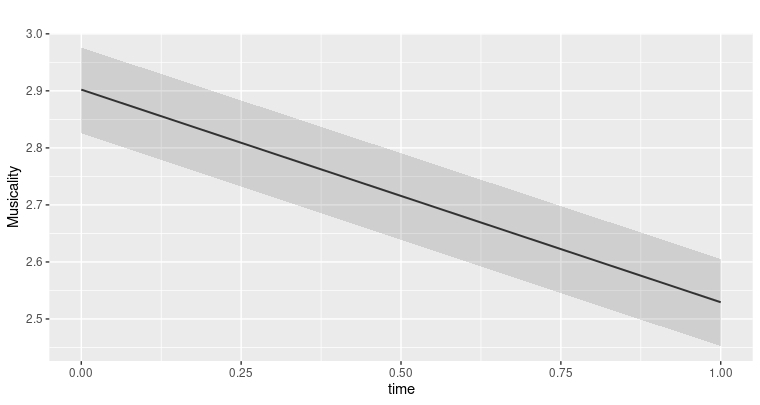
\includegraphics[width=15cm,height=10cm,keepaspectratio]{Musicality}
	\caption{Predicted Values of \textit{Musicality} over time}
	\label{fig:mus}
\end{figure}

The results further revealed only a few demographic predictors that influenced participants' \textit{musicality} scores. Initially, younger participants scored slightly higher in \textit{musicality} (-0.08, [-0.18, 0.01]). Partcipants with higher cognitive reserve scores achieved better overall scores (0.10, [0.01, 0.19]). Aditionally, participants with higher CogTel scores obtained higher \textit{musicality} scores (0.08, [0.00, 0.18]). The effect sizes are small but clear.
Over time, participants with more cognitive reserve and higher CogTel scores showed less decrease in \textit{musicality} scores (cogntive reserve: 0.19, [0.06, 0.32]; CogTel: 0.19, [0.07, 0.32]). Similarly, the scores of younger (-0.22, [-0.35, -0.09]) and male (0.2, [0.09, 0.32]) participants diminished less. Participants with higher income and those who spent more time on their homework also experienced a smaller decrease in \textit{musicality} scores (income: 0.16, [0.03, 0.29]; homework: 0.34, [0.21, 0.47]). Moreover, participants who were less engaged in musical activities and had fewer emotions towards music demonstrated a lower decrease of \textit{musicality} scores after the intervention with the easy version of "Ode to Joy" (Musical Engagement: -0.25, [-0.38, -0.11]; Emotions: -0.37 [-0.49, -0.24]). Better singing abilities and more general sophistication in music also minimized the decrease of \textit{musicality} over time (Singing abilities: -0.25, [-0.38, -0.12]; general sophistication: -0.18, [-0.31, -0.05]). 
In the more challenging version of "Ode to Joy", participants with higher education (0.2, [0.06, 0.34]), higher perceptual abilities (0.36, [0.22, 0.5]), higher CogTel scores (0.26, [0.11,0.4]) and more cognitive reserve (0.47, [0.33, 0.61]) performed better compared to other participants. Participants from Hannover (-0.31, [-0.45, -0.17]) and those who spent more time doing homework (0.23, [0.08, 0.28]) had a positive impact on musical performance. Additionally, better singing abilities and greater general sophistication in music also positively influenced \textit{musicality} scores after the intervention with the challenging version of "Ode to Joy" (0.19, [0.05, 0.34]; 0.26, [0.12, 0.41]).



%\section{?? Progress of Musical Abilities}
%\subsection{BAT, MDT, Scales}
%\subsection{GoldMSI}

